% Calculus homework (English, university), with a tikz sketch.
% Headings: run-in "Problem N. (Title, P points)" followed directly by the statement; parts (a), (b), ...
\documentclass[11pt,a4paper]{article}
\usepackage[T1]{fontenc}
\usepackage{lmodern}
\usepackage[margin=2.3cm,top=2.0cm,bottom=2.2cm]{geometry}
\usepackage{amsmath,amssymb}
\usepackage{siunitx}
\usepackage{tikz}
\usetikzlibrary{arrows.meta,decorations.pathmorphing}
\usepackage{enumitem}

\setlength{\parindent}{0pt}
\setlist[enumerate,1]{label=(\alph*), leftmargin=2.2em, itemsep=0.4em, topsep=0.3em}
% run-in heading: the statement follows on the same line
\newcommand{\problem}[3]{\bigskip\par\textbf{Problem #1.} (#2, #3 points)\ }
\newcommand{\dd}{\,\mathrm{d}}

\begin{document}

% ---- header ---------------------------------------------------------------------------
{\small MATH 1101 \textperiodcentered{} Calculus I \hfill Department of Mathematics}\\[-0.4em]
\rule{\linewidth}{0.6pt}\\[0.5em]
{\Large\bfseries Homework 8}\\[0.4em]
Due: Monday, November 17, 2026, at the start of lecture \hfill Total: 36 points\\[0.3em]
{\small Justify your answers. Give exact values unless a decimal approximation is asked for.}

% ---- Problem 1 ------------------------------------------------------------------------
\problem{1}{Limits}{8}Evaluate the following limits, or explain why they do not exist.
\begin{enumerate}
  \item $\displaystyle\lim_{x\to 2}\frac{x^2-4}{x-2}$
  \item $\displaystyle\lim_{x\to 0}\frac{\sin(3x)}{2x}$
  \item $\displaystyle\lim_{x\to\infty}\left(\sqrt{x^2+x}-x\right)$
  \item $\displaystyle\lim_{x\to 0}\frac{e^x-1-x}{x^2}$
\end{enumerate}

% ---- Problem 2 ------------------------------------------------------------------------
\problem{2}{Derivatives}{8}Differentiate each function. Use the chain rule and the product rule where needed.
\begin{enumerate}
  \item $f(x) = (3x^2+1)^5$
  \item $g(x) = x^2 e^{-x}$
  \item $h(x) = \sin(x^2)\,\ln x$ for $x>0$
  \item Find the equation of the tangent line to the graph of $g$ from part (b) at $x=1$.
\end{enumerate}

% ---- Problem 3 ------------------------------------------------------------------------
\problem{3}{Substitution}{6}Evaluate the integrals using a suitable substitution.
\begin{enumerate}
  \item $\displaystyle\int x\,e^{x^2}\dd x$
  \item $\displaystyle\int_0^1 x\sqrt{1+x^2}\dd x$
  \item $\displaystyle\int_1^e \frac{\ln x}{x}\dd x$
\end{enumerate}

% ---- Problem 4 ------------------------------------------------------------------------
\problem{4}{Optimisation}{8}A farmer has \SI{120}{m} of fencing and wants to enclose a rectangular
field next to a straight river. No fence is needed along the river. The field is divided into two equal
pens by one more fence perpendicular to the river, as in the sketch. Let $x$ be the length of each
fence perpendicular to the river and $y$ the length of the field along the river.

\begin{center}
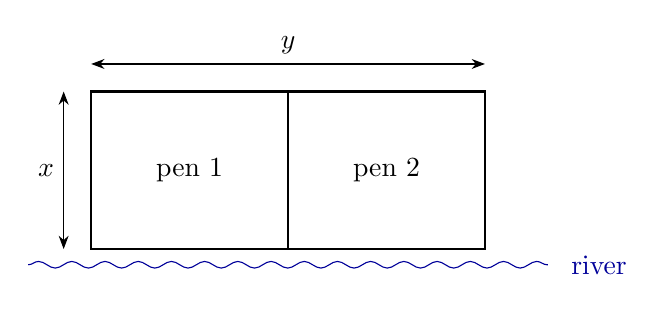
\begin{tikzpicture}[>=Stealth]
  \draw[thick] (0,0) rectangle (5,2);
  \draw[thick] (2.5,0) -- (2.5,2);
  % the river along the bottom
  \draw[blue!60!black, decorate, decoration={snake, amplitude=1.2pt, segment length=12pt}] (-0.8,-0.2) -- (5.8,-0.2);
  \node[blue!60!black] at (6.45,-0.2) {river};
  \draw[<->] (-0.35,0) -- (-0.35,2) node[midway, left] {$x$};
  \draw[<->] (0,2.35) -- (5,2.35) node[midway, above] {$y$};
  \node at (1.25,1) {pen 1};
  \node at (3.75,1) {pen 2};
\end{tikzpicture}
\end{center}
\begin{enumerate}
  \item Express the enclosed area $A$ as a function of $x$ alone and state its domain.
  \item Find the value of $x$ that maximises $A$, and use the second derivative to confirm that it is a
        maximum.
  \item What are the dimensions of the field and the maximal area?
\end{enumerate}

% ---- Problem 5 ------------------------------------------------------------------------
\problem{5}{Taylor polynomial}{6}Let $f(x) = \ln(1+x)$.
\begin{enumerate}
  \item Find the Taylor polynomial $T_3$ of degree $3$ of $f$ about $x_0 = 0$.
  \item Use $T_3$ to approximate $\ln(1.2)$.
  \item Use the Lagrange form of the remainder to give an upper bound for the error of your
        approximation in part (b).
\end{enumerate}

\end{document}
